\documentclass[a4paper]{article}
\usepackage[german]{babel}
%\usepackage{libertine}
%\renewcommand*\familydefault{\sfdefault}  %%
\usepackage[default]{opensans}
%\usepackage{gillius2}
%\usepackage{lato}
\usepackage[version=4]{mhchem}

\usepackage[utf8]{inputenc}

\usepackage[T1]{fontenc}

%\usepackage[activate={true,nocompatibility},final,tracking=true,kerning=true,spacing=true,factor=1100,stretch=10,shrink=10]{microtype}

\usepackage[utf8]{inputenc}
\usepackage[T1]{fontenc}

\usepackage{libertine}
\usepackage{microtype}

\usepackage{xcolor,multido}
\usepackage{tikz}
\usepackage{pgffor}
\usepackage{graphicx}
\usepackage[left=1cm,right=1cm,top=1.5cm,bottom=2cm]{geometry}



\begin{document}
\begin{tikzpicture}
\node[inner sep=0pt] (russell) at (0,0)
    {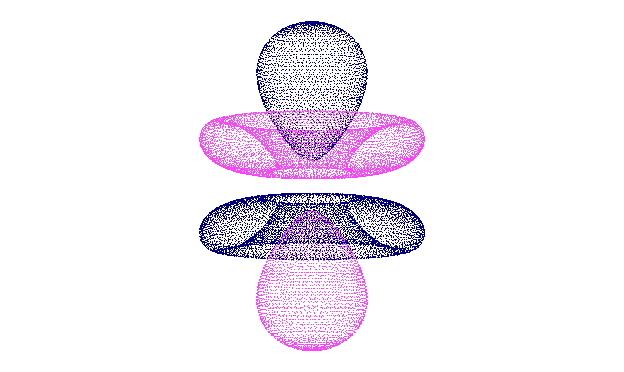
\includegraphics[width=\textwidth]{fg0.png}};
    % The axes
\draw[->,ultra thick] (xyz cs:x=-6.5) -- (xyz cs:x=6.5) node[above] {\Large x};
\draw[->,ultra thick] (xyz cs:y=-6.5) -- (xyz cs:y=6.5) node[right] {\Large y};
\draw[->,ultra thick] (xyz cs:z=-6.5) -- (xyz cs:z=6.5) node[above] {\Large z};
%\node[inner sep=0pt] (whitehead) at (5,-6)
 %   {\includegraphics[width=.25\textwidth]{alfred_north_whitehead.jpg}};
%\draw[<->,thick] (russell.south east) -- (whitehead.north west)
 %   node[midway,fill=white] {Principia Mathematica};
\end{tikzpicture}

\begin{tikzpicture}
\node[inner sep=0pt] (russell) at (0,0)
    {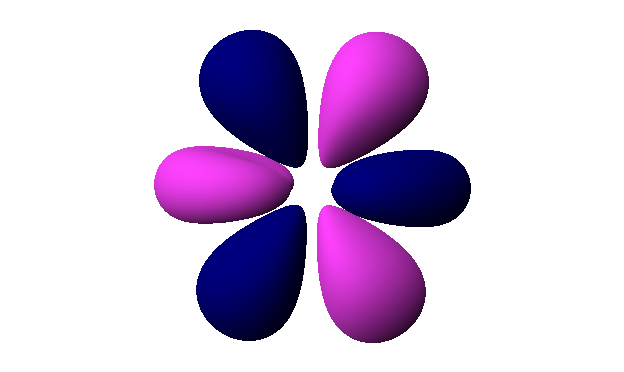
\includegraphics[width=\textwidth]{fg1.png}};
    % The axes
\draw[->,ultra thick] (xyz cs:x=-6.5) -- (xyz cs:x=6.5) node[above] {\Large x};
\draw[->,ultra thick] (xyz cs:y=-6.5) -- (xyz cs:y=6.5) node[right] {\Large y};
\draw[->,ultra thick] (xyz cs:z=-6.5) -- (xyz cs:z=6.5) node[above] {\Large z};
%\node[inner sep=0pt] (whitehead) at (5,-6)
 %   {\includegraphics[width=.25\textwidth]{alfred_north_whitehead.jpg}};
%\draw[<->,thick] (russell.south east) -- (whitehead.north west)
 %   node[midway,fill=white] {Principia Mathematica};
\end{tikzpicture}

%\draw (0.2,0) circle (2mm); & \fill[red] (0,0) circle (3mm); \\};

%\draw (0.4,0) circle (2mm); & \fill[red] (0,4) circle (3mm); \\
%\draw [very thick,->] (0,0) |- (my matrix.west);

\end{document}